%\noindent {\it Example:  all transitive permutation representations of $A_5$.}\\[4pt]
\gap\ has a function for determining the conjugacy classes of
subgroups, which we now use to find (up to equivalence) all permutation
representations of the group $A_5$.
First, we define the alternating group on five points, and then
compute the conjugacy classes of subgroups.\footnote{Note: {\tt
    ConjugacyClassesSubgroups} does not compute the ordinary conjugacy classes of
  elements of the group. (Those are found with the command {\tt ConjugacyClasses}.)
  Rather, {\tt ConjugacyClassesSubgroups( G )} partitions the set $\Sub[G]$ of
  subgroups of $G$ into conjugacy classes \emph{of subgroups}.} 

{\codesize 
\begin{verbatim}

gap> a5 := AlternatingGroup(5);;
gap> ccls := ConjugacyClassesSubgroups( a5 );
[ Group( () )^G, Group( [ (2,3)(4,5) ] )^G, Group( [ (3,4,5) ] )^G, 
  Group( [ (2,3)(4,5), (2,4)(3,5) ] )^G, Group( [ (1,2,3,4,5) ] )^G, 
  Group( [ (3,4,5), (1,2)(4,5) ] )^G, Group( [ (1,2,3,4,5), (2,5)(3,4) ] )^G, 
  Group( [ (2,3)(4,5), (2,4)(3,5), (3,4,5) ] )^G, 
                   AlternatingGroup( [ 1 .. 5 ] )^G ]

\end{verbatim}}

\noindent If you are running \xgap, an extension of \gap, you can see a diagram of the entire
subgroup lattice of a group (of reasonably small order).  For example, at the {\tt
  xgap} command line we could type {\tt GraphicSubgroupLattice( a5 )}.  This opens a
new window showing just the two subgroups $(e)$ and $A_5$.  Selecting {\tt All
  Subgroups} from the {\tt Subgroups} drop-down menu draws a (rather messy) Hasse
diagram of $\Sub[A_5]$.  You can then move around the various conjugacy classes of
subgroups (which stayed glued together) to get a pretty good picture of
$\Sub[A_5]$. (See Figure~\ref{fig:A5new}.)

\begin{figure}[h!]
%\scaling{20}%
\begin{center}
\vspace{-5cm}
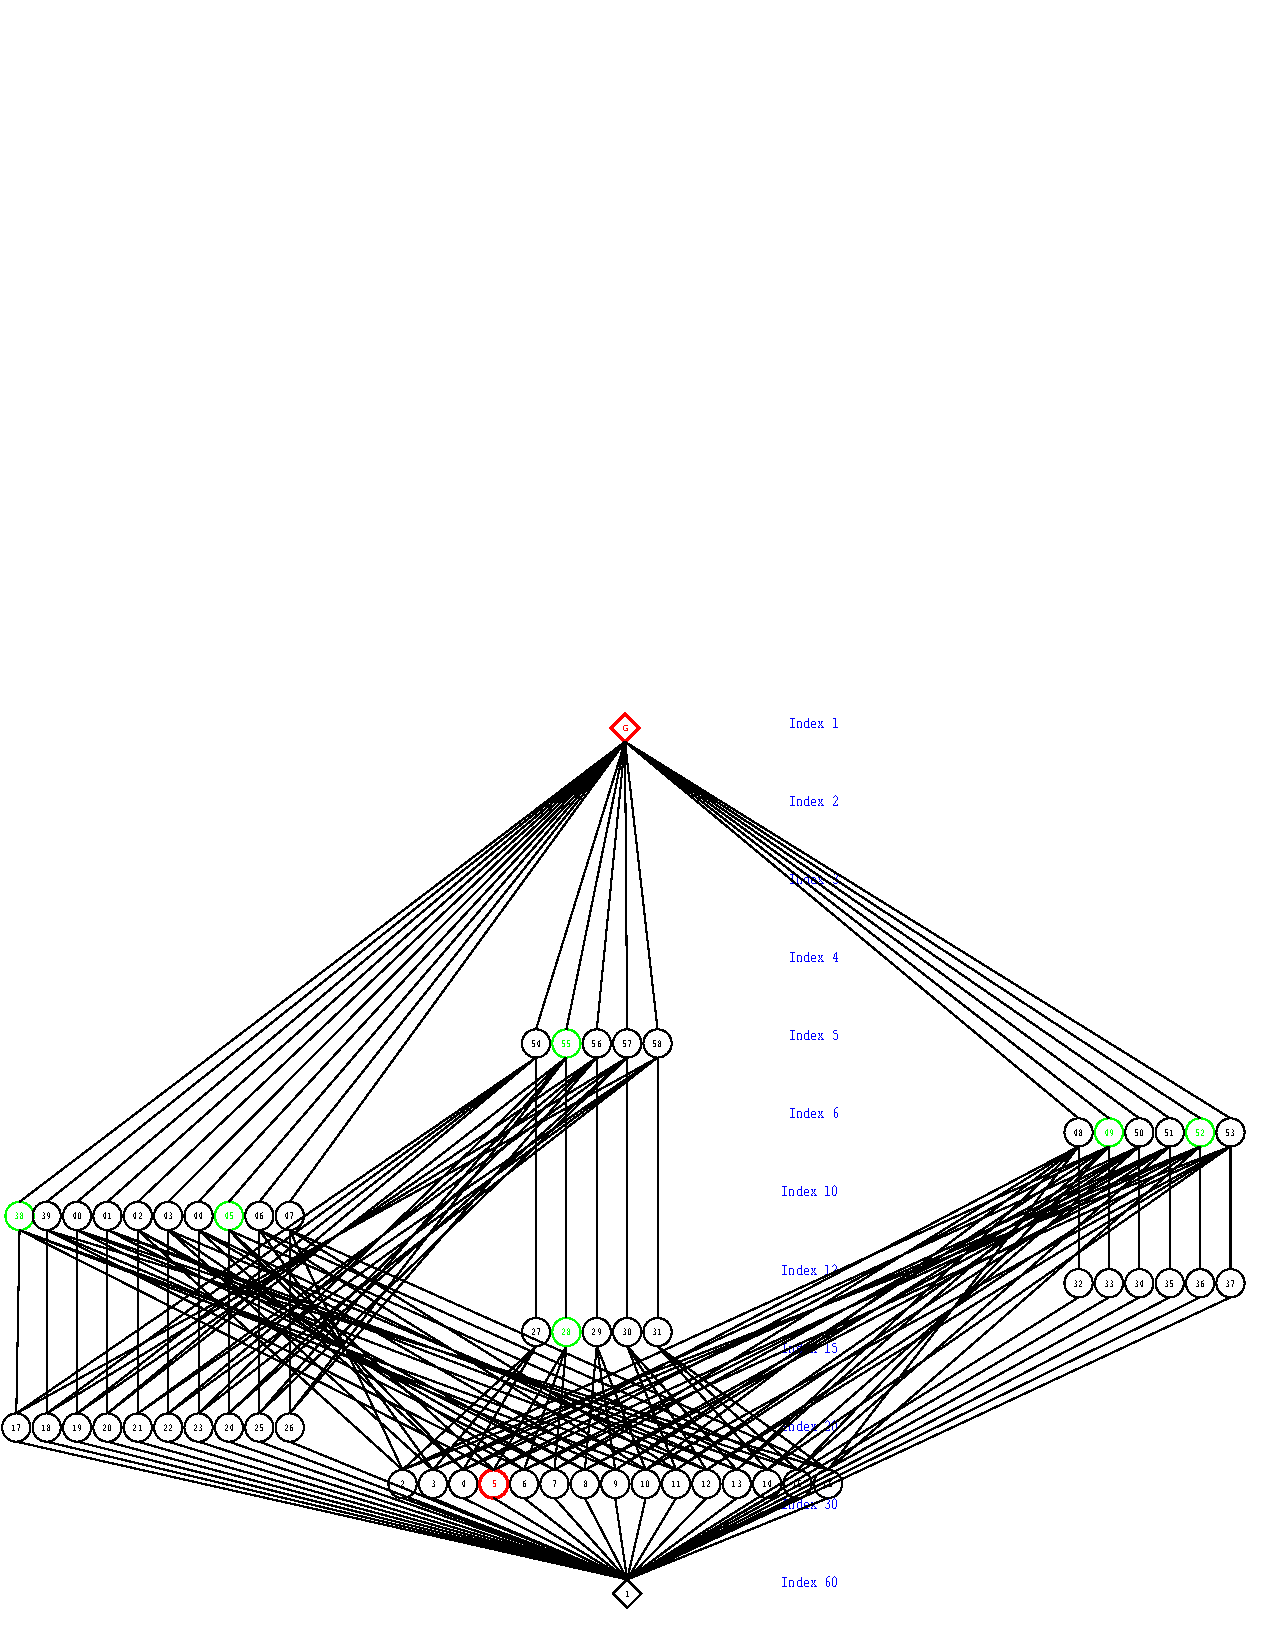
\includegraphics[height=13cm]{A5UpperN5.pdf}%
\caption{Hasse diagram of $\Sub[A_5]$ drawn by the \xgap\ program. Colored green are the
subgroups in the interval above one of the $\Z_2$ subgroups of $A_5$.  Thus,
$A_5$ acts transitively on the 30 cosets of $\Z_2$, and the
permutational algebra $\<A_5/\Z_2; A_5\>$ has congruence lattice isomorphic to 
the interval $[\Z_2, A_5]$.}
\label{fig:A5new}
\end{center}
\end{figure}

If we use the \xgap\ program as described above we could count the conjugacy classes of subgroups by
looking at the Hasse diagram of $\Sub[A_5]$.  However, it's more convenient (and
faster) to simply do: 
{\codesize 
\begin{verbatim}
gap> ccsg := ConjugacyClassesSubgroups( a5 );;
gap> Size(ccsg);
\end{verbatim}}
\noindent which returns 9, telling us that $A_5$ has 9 conjugacy classes of subgroups.  
This includes the singleton classes $\{(e)\}$ and $\{A_5\}$,
which \gap\ calls \verb!Group( () )^G! and \verb!AlternatingGroup( [ 1 .. 5 ] )^G!,
respectively. 
Let's examine the other seven classes.  We get a list of representative subgroups, one for
each class, as follows:
{\codesize 
\begin{verbatim}

gap> clreps := List( ccsg, x -> Representative( x ));
[ Group(()), Group([ (2,3)(4,5) ]), Group([ (3,4,5) ]), 
  Group([ (2,3)(4,5), (2,4)(3,5) ]), Group([ (1,2,3,4,5) ]), 
  Group([ (3,4,5), (1,2)(4,5) ]), Group([ (1,2,3,4,5), (2,5)(3,4) ]), 
  Group([ (2,3)(4,5), (2,4)(3,5), (3,4,5) ]), Alt( [ 1 .. 5 ] ) ]

\end{verbatim}}
\noindent The orders and indices of these subgroups are given by
{\codesize 
\begin{verbatim}

gap> List( clreps, x -> Order(x));         
     % returns [ 1, 2, 3, 4, 5, 6, 10, 12, 60 ]
gap> List( clreps, x -> Index( a5, x ) );  
     % returns [ 60, 30, 20, 15, 12, 10, 6, 5, 1 ]

\end{verbatim}}
\noindent (Of course, any subgroup $H\leq A_5$ has order $|H| = |A_5|\,[A_5:H] = 60 \,[A_5:H]$.)  
From the list of subgroup orders, we see that {\tt clreps[2]}, {\tt clreps[3]},
and {\tt clreps[5]} must be the groups $\Z_2$, $\Z_3$, and $\Z_5$ (the only groups of 
orders two, three, and five, respectively).  
We can easily identify the other subgroups as well.\footnote{A
  nice reference list of all groups of orders 1 through 15 is given on pp.~98--9 of
  Hungerford~\cite{Hungerford:1974}.} 
For example, {\tt clreps[4]} has order 4, so it must be either 
$\Z_2 \oplus \Z_2$ or $\Z_4$.  Deciding to which isomorphism class {\tt clreps[4]}
belongs is simply a matter of checking whether it's cyclic.  These and other
subgroups can be determined using the following \gap\ commands:
% {\tt IsCyclic}, {\tt IsAbelian}, {\tt IsDihedralGroup}, {\tt IsAlternatingGroup}; e.g.
{\codesize 
\begin{verbatim}

gap> IsCyclic( clreps[4] );            # returns false
gap> IsAbelian( clreps[6] );           # returns false
gap> IsDihedralGroup( clreps[6] );     # returns true
gap> IsDihedralGroup( clreps[7] );     # returns true
gap> IsAlternatingGroup( clreps[8] );  # returns true

\end{verbatim}}
\noindent Therefore, {\tt clreps[4]} must be the Klein four group $\Z_2 \oplus
\Z_2$, {\tt clreps[6]} must be $D_3$, 
{\tt clreps[7]}  must be $D_5$.  Finally, {\tt clreps[8]} has
order 12, so it must be one of $\Z_2 \oplus \Z_{6}$, $\Z_{12}$, $A_4$,
$D_6$, or %$T$.
the group $T$ (generated by two elements $a, b$ where $|a|=6, b^2 = a^3$, and $ba = a^{-1}b$).  
The last command above shows that {\tt clreps[8]} is $A_4$.

The foregoing demonstrates some useful \gap\ commands, but we could have
identified all these subgroups in one step with the {\tt StructureDescription} command:
{\codesize 
\begin{verbatim}

gap> List(clreps, x->StructureDescription(x));
[ "1", "C2", "C3", "C2 x C2", "C5", "S3", "D10", "A4", "A5" ]

\end{verbatim}}

Now, the representations of $A_5$ are all faithful since $A_5$ is simple.  Below is
a table of all seven (equivalence classes of) permutation representations of
$A_5$ on cosets $A_5/H$, ordered by the number of such cosets (i.e.~the index
$[A_5:H]$): \\
{\small
  \begin{center}
\begin{tabular}{c|c|c|c}
%Conjugacy class & Index & & \\
  Conjugacy & Index & &  \\
   class rep.~$H$   & $[A_5: H]$ & Representation homomorphism & Is it primitive?\\
\hline
$A_4$ &  5 & $\rho_{A_4}  : A_5 \hookrightarrow \Sym(A_5/A_4) \cong S_5$ & yes \\
$D_5$ &  6 & $\rho_{D_5}  : A_5 \hookrightarrow \Sym(A_5/D_5) \cong S_6$ & yes \\
$D_3$ & 10 & $\rho_{D_3}  : A_5 \hookrightarrow \Sym(A_5/D_3) \cong S_{10}$ & yes \\
$\Z_5$& 12 & $\rho_{\Z_5} : A_5 \hookrightarrow \Sym(A_5/\Z_5) \cong S_{12}$ & no\\
$V_4$ & 15 & $\rho_{V_4}  : A_5 \hookrightarrow \Sym(A_5/V_4) \cong S_{15}$ & no\\
$\Z_3$& 20 & $\rho_{\Z_3} : A_5 \hookrightarrow \Sym(A_5/\Z_3) \cong S_{20}$ & no\\
$\Z_2$& 30 & $\rho_{\Z_2} : A_5 \hookrightarrow \Sym(A_5/\Z_2) \cong S_{30}$ & no\\
$(e)$& 60 & $\rho : A_5 \hookrightarrow \Sym(A_5) \cong S_{60}$ & no\\
\hline
\end{tabular}
  \end{center}
  }
~\\[4pt]
We can use \gap\ to verify that $A_5$ does indeed show up as a transitive
subgroup of some of the symmetric groups listed in the table above.  For
example, the first two are checked as follows:
{\codesize 
\begin{verbatim}

gap> NrTransitiveGroups(5);  % returns 5
gap> NrTransitiveGroups(6);  % returns 16
gap> List([1..5], x->StructureDescription(TransitiveGroup(5,x)));
[ "C5", "D10", "C5 : C4", "A5", "S5" ]
gap> List([1..16], x->StructureDescription(TransitiveGroup(6,x)));
[ "C6", "S3", "D12", "A4", "C3 x S3", "C2 x A4", "S4", "S4", "S3 x S3", 
  "(C3 x C3) : C4", "C2 x S4", "A5", "(S3 x S3) : C2", "S5", "A6", "S6" ]

\end{verbatim}}
\noindent The last line above indicates that (some copy of) $A_5$ shows up as a transitive
subgroup of $S_6$.  (Of course, it is \emph{not} the copy of $A_5< S_6$ that
moves only five points!) 

The last column of the table above was filled in simply 
by looking at the subgroup lattice of $A_5$ in~Figure~\ref{fig:A5new}.  
In general, if $H$ is a coatom in $\Sub[G]$ (i.e.~a maximal subgroup of $G$),
then the representation  
\[
\rho_{H} : G \rightarrow \Sym(G/H) \cong S_{[G:H]}
\] is primitive.
\\[10pt]
{\bf G-sets.} Defining G-sets with \gap\ is very useful and important.  It allows us to work
with and analyze a particular permutation representation.  Let us consider the
$A_5$-set given by $A_5$ acting on cosets of $H=$ {clreps[2]} $=C_2$. In \gap\
we do
{\codesize 
\begin{verbatim}

gap> G := AlternatingGroup( 5 );;
gap> ccsg := ConjugacyClassesSubgroups( a5 );;
gap> H := Representative( ccsg[3] );                   # C3
gap> Gbar := Action( G, RightCosets(G,H), OnRight );;  # a subgroup of S20 
                                                       # isomorphic to A5
gap> MovedPoints( Gbar );                              # [ 1, ..., 20 ]
gap> AllBlocks( Gbar );    # [ [ 1, 2, 3, 4 ], [ 1, 6, 11, 16 ], [ 1, 20 ] ]
gap> for b in AllBlocks( Gbar ) do Print( Orbit( Gbar, b, OnSets ), "\n"); od;
\end{verbatim}}
{\scriptsize 
\begin{verbatim}
[[ 1, 2, 3, 4 ], [ 17, 18, 19, 20 ], [ 13, 14, 15, 16 ], [ 9, 10, 11, 12 ], [ 5, 6, 7, 8 ]]
[[ 1, 6, 11, 16 ], [ 2, 7, 12, 17 ], [ 3, 8, 13, 18 ], [ 4, 9, 14, 19 ], [ 5, 10, 15, 20 ]]
[[ 1, 20 ], [ 16, 17 ], [ 12, 13 ], [ 11, 18 ], [ 8, 9 ], [ 7, 14 ], [ 6, 19 ], ...
  ..., [ 4, 5 ], [ 3, 10 ], [ 2, 15 ]]

\end{verbatim}}
\noindent The command {\tt MovedPoints} shows that {\tt Gbar} $\cong A_5$ acts transitively on the set
$G/H = A_5/Z_3$ of 30 cosets.  (We could also have checked that the action is transitive
using {\tt Orbits(Gbar)} and noting that there is just one orbit.)
The command {\tt AllBlocks(Gbar)} shows 
the first block of each nontrivial ``system of imprimitivity'' (or congruence) of
the G-set $\<G/H, \bar{G}\>$.  Finally, the last command displays the three
nontrivial congruences, and shows $\Con \<G/H, \bar{G}\>\cong M_3$.  Another way
to see that  $\Con \<G/H, \bar{G}\>\cong M_3$ is to check the sublattice of
intermediate subgroups between $H$ and $G$, as follows:
{\codesize 
\begin{verbatim}
gap> intHG := IntermediateSubgroups(G, H);
\end{verbatim}}
{\codesize
\begin{verbatim}
rec( subgroups := [ Group([(3,4,5), (1,2)(4,5)]), Group([(3,4,5), (2,3)(4,5)]), 
                    Group([(3,4,5), (1,5,3)]) ], 
     inclusions := [[ 0, 1 ], [ 0, 2 ], [ 0, 3 ], [ 1, 4 ], [ 2, 4 ], [ 3, 4 ]] 
   )
\end{verbatim}}
\noindent This results in an object, which I've called {\tt intHG}, having fields
{\tt intHG.subgroups} and {\tt intHG.inclusions}.  The inclusions field shows
the covering relations in the sublattice interval $[H, G] \leq \Sub[G]$.

  % \\[6pt]
% {\bf A more general example.}  The example above was special because $A_5$ is a
% simple group.  In general, given a finite group $G$, and an arbitrary subgroup
% $H$, the representation $\rho_H$ need not be an embedding of $G$ into
% $\Sym(G/H)$.  
